\documentclass{beamer}
\usepackage[french]{babel}

\mode<presentation> {

% The Beamer class comes with a number of default slide themes
% which change the colors and layouts of slides. Below this is a list
% of all the themes, uncomment each in turn to see what they look like.

%\usetheme{default}
%\usetheme{AnnArbor}
%\usetheme{Antibes}
%\usetheme{Bergen}
%\usetheme{Berkeley}
%\usetheme{Berlin}
%\usetheme{Boadilla}
%\usetheme{CambridgeUS}
%\usetheme{Copenhagen}
%\usetheme{Darmstadt}
%\usetheme{Dresden}
%\usetheme{Frankfurt}
%\usetheme{Goettingen}
%\usetheme{Hannover}
%\usetheme{Ilmenau}
%\usetheme{JuanLesPins}
%\usetheme{Luebeck}
\usetheme{Madrid}
%\usetheme{Malmoe}
%\usetheme{Marburg}
%\usetheme{Montpellier}
%\usetheme{PaloAlto}
%\usetheme{Pittsburgh}
%\usetheme{Rochester}
%\usetheme{Singapore}
%\usetheme{Szeged}
%\usetheme{Warsaw}

% As well as themes, the Beamer class has a number of color themes
% for any slide theme. Uncomment each of these in turn to see how it
% changes the colors of your current slide theme.

%\usecolortheme{albatross}
%\usecolortheme{beaver}
%\usecolortheme{beetle}
%\usecolortheme{crane}
%\usecolortheme{dolphin}
%\usecolortheme{dove}
%\usecolortheme{fly}
%\usecolortheme{lily}
%\usecolortheme{orchid}
%\usecolortheme{rose}
%\usecolortheme{seagull}
%\usecolortheme{seahorse}
%\usecolortheme{whale}
%\usecolortheme{wolverine}

%\setbeamertemplate{footline} % To remove the footer line in all slides uncomment this line
%\setbeamertemplate{footline}[page number] % To replace the footer line in all slides with a simple slide count uncomment this line

%\setbeamertemplate{navigation symbols}{} % To remove the navigation symbols from the bottom of all slides uncomment this line
}

\usepackage{graphicx} % Allows including images
\usepackage{booktabs} % Allows the use of \toprule, \midrule and \bottomrule in tables
\usepackage[utf8]{inputenc}
\usepackage{bm}

%----------------------------------------------------------------------------------------
%	TITLE PAGE
%----------------------------------------------------------------------------------------

\title[Effet bilame]{Effet bilame (bimetallic strip)}
\author[Groupe 4]{Fakri Yassir, Karroucha Wissam, Mazé François, Pollet Florent} % Your name
\institute[Mines Paris] % Your institution as it will appear on the bottom of every slide, may be shorthand to save space
{
Mines ParisTech \\ % Your institution for the title page
}
\date{\today} % Date, can be changed to a custom date

\begin{document}
\begin{frame}
\titlepage % Print the title page as the first slide
\begin{figure}
    \centering
    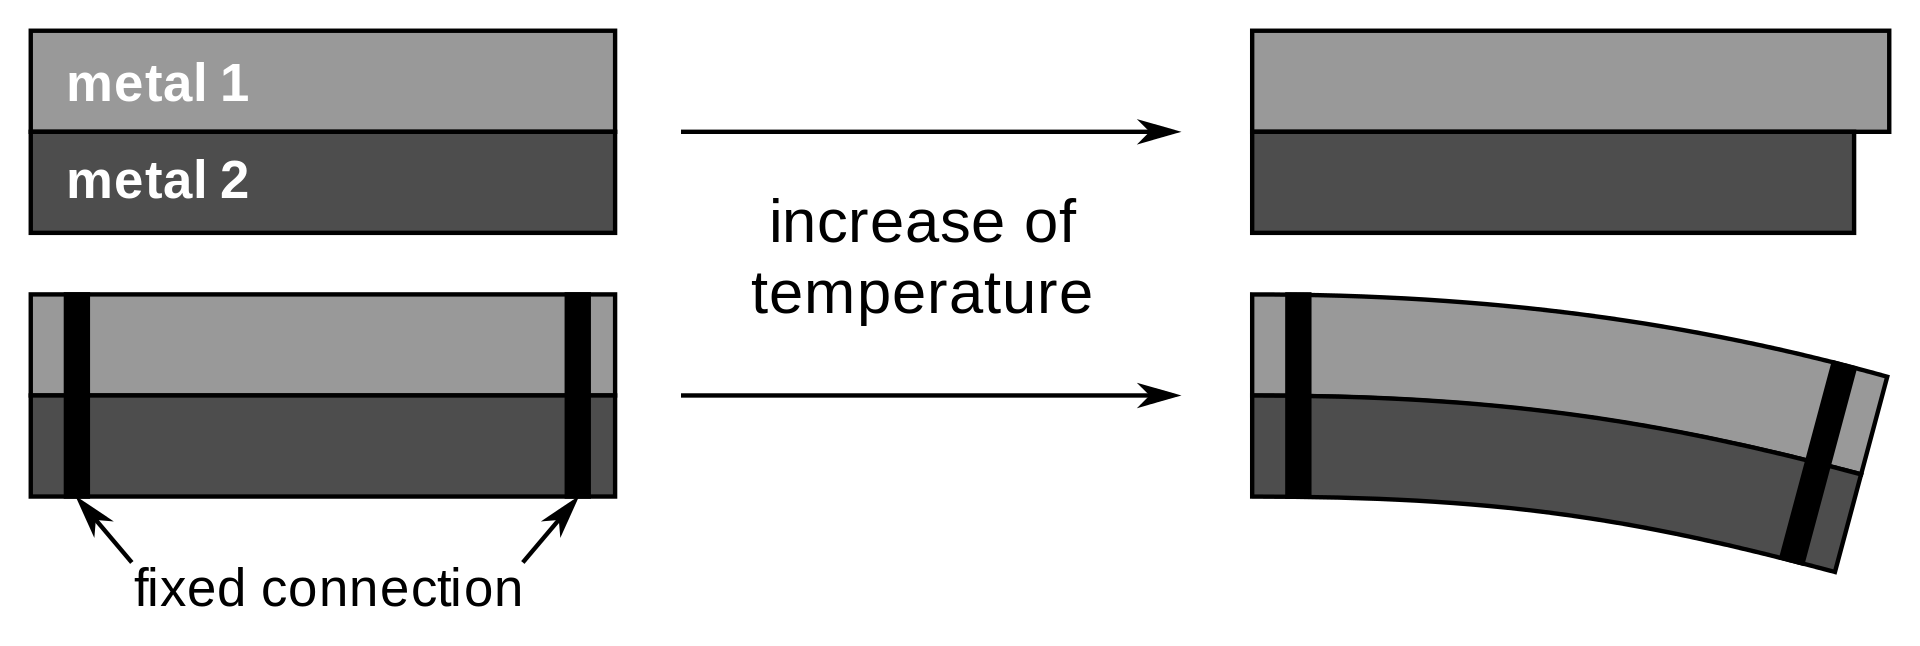
\includegraphics[scale=0.1]{imgs/bilame.png}
\end{figure}
\end{frame}

\begin{frame}
\frametitle{Plan} % Table of contents slide, comment this block out to remove it
\tableofcontents % Throughout your presentation, if you choose to use \section{} and \subsection{} commands, these will automatically be printed on this slide as an overview of your presentation
\end{frame}

%----------------------------------------------------------------------------------------
%	PRESENTATION SLIDES
%----------------------------------------------------------------------------------------
\section{Effet bilame} % Sections can be created in order to organize your presentation into discrete blocks, all sections and subsections are automatically printed in the table of contents as an overview of the talk
%------------------------------------------------

\subsection{Contraintes équi-biaxiales} 
\subsection{Déformations des couches} 
\subsection{Equations de compatibilité} 
\subsection{Déplacements} 
\subsection{Contraintes dans chaque couche} 
\subsection{Torseur des efforts résultant}

\begin{frame}
    \frametitle{Torseur des efforts résultants}
    On se place sur un élément de la surface latérale $\partial S \times ]-h_s,h_f[$, de largeur infinitésimale $dl$ :
    \begin{figure}
        \centering
        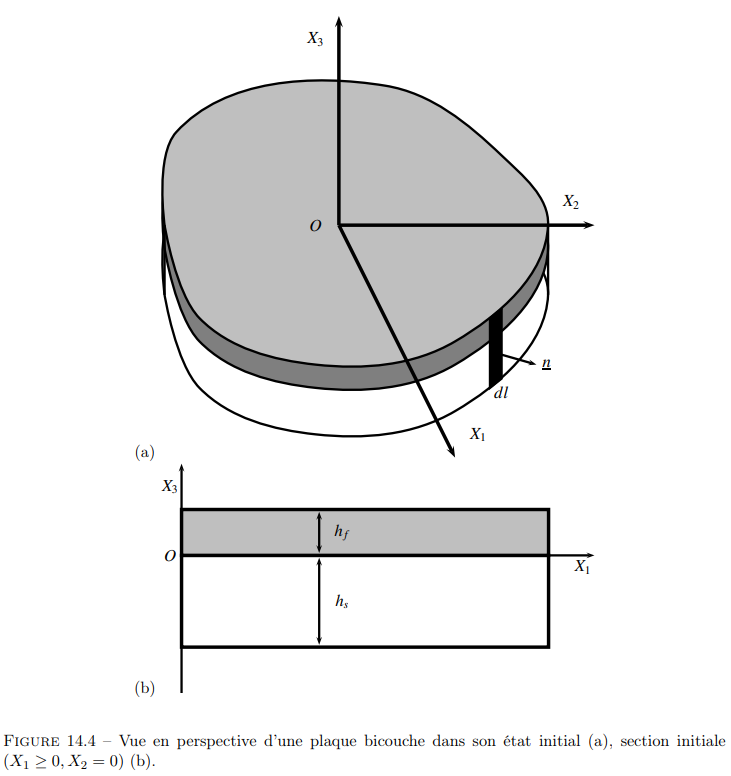
\includegraphics[scale=0.5]{imgs/surface_etude.png}
    \end{figure}
\end{frame}

\begin{frame}
    \frametitle{Torseur des efforts résultants}
    En notant $\partial S_l$ le contour de largeur $dl$, on a donc la résultante suivante des efforts surfaciques :
    $$\underline{R^{s}} = \int_{\partial S_l \times ]-h_s,h_f[}\underline{t}\;ds = \int_{\partial S_l \times ]-h_s,h_f[}\underset{\sim}{\sigma}\cdot\underline{n}\;dl\;dX_3$$
    On introduit la résultante linéique, en divisant par la largeur $dl$ :
    $$\underline{R} = \int_{-h_s}^{h_f}\underset{\sim}{\sigma}\cdot\underline{n}\;dX_3$$
    $n_3 = 0$ donc $R_3 = 0$. On calcule $R_1$ et $R_2$ :
    $$R_1 = \int_{-h_s}^{h_f}\sigma_{11}\;n_1\;dX_3 = (\int_{-h_s}^{h_f}\sigma_{11}\;dX_3)n_1$$
    $$R_2 = \int_{-h_s}^{h_f}\sigma_{22}\;n_2\;dX_3 = (\int_{-h_s}^{h_f}\sigma_{22}\;dX_3)n_2$$
\end{frame}

\begin{frame}
    \frametitle{Torseur des efforts résultants}
    On calcule aussi le moment résultant des efforts surfaciques, par rapport au point $O$ :
    $$\underline{M^{s}} = \int_{\partial S_l \times ]-h_s,h_f[}\underline{X}\wedge \underline{t}\;ds$$
    On introduit de même la résultante linéique, en divisant par la largeur $dl$ :
    $$\underline{M} = \int_{-h_s}^{h_f}\underline{X}\wedge (\underset{\sim}{\sigma}\cdot\underline{n})\;dX_3 = \int_{-h_s}^{h_f}\begin{pmatrix} X_1 \\ X_2 \\ X_3 \end{pmatrix}\wedge \begin{pmatrix} \sigma_{11}\;n_1 \\ \sigma_{22}\;n_2 \\ 0 \end{pmatrix}\;dX_3$$
    D'où $$\underline{M} = \int_{-h_s}^{h_f}\begin{pmatrix} -X_3\;\sigma_{22}\;n_2 \\ \sigma_{11}\;n_1\;X_3 \\ \sigma_{22}\;X_1\;n_2 - X_2\;\sigma_{11}\;n_1 \end{pmatrix}\;dX_3$$
\end{frame}

\begin{frame}
    \frametitle{Torseur des efforts résultants}
    Pour récapituler :
    $$R_1 = (\int_{-h_s}^{h_f}\sigma_{11}\;dX_3)n_1$$
    $$R_2 = (\int_{-h_s}^{h_f}\sigma_{22}\;dX_3)n_2$$
    $$M_1 = (\int_{-h_s}^{h_f} -X_3\;\sigma_{11}\;dX_3)n_2$$
    $$M_2 = (\int_{-h_s}^{h_f} X_3\;\sigma_{11}\;dX_3)n_1$$
    $$M_3 = (n_2\;X_1\;\int_{-h_s}^{h_f} \sigma_{11}\;dX_3 - n_1\;X_2 \int_{-h_s}^{h_f} \sigma_{11}\;dX_3$$
    Il suffit de calculer $\int_{-h_s}^{h_f}\sigma_{11}\;dX_3$ et $\int_{-h_s}^{h_f}X_3\;\sigma_{11}\;dX_3$ !
\end{frame}

\begin{frame}
    \frametitle{Torseur des efforts résultants}
    D'une part :
    $$\int_{-h_s}^{h_f}\sigma_{11}\;dX_3$$ $$=\int_{-h_s}^{0}M_s(AX_3+C-\alpha_s(T-T_0))\;dX_3+\int_{0}^{h_f}M_f(AX_3+C-\alpha_f(T-T_0))\;dX_3$$
    $$=-M_sA\frac{h_s^{2}}{2}+M_s(C-\alpha_s(T-T_0))h_s+M_fA\frac{h_f^{2}}{2}+M_f(C-\alpha_f(T-T_0))h_f$$
    D'autre part :
    $$\int_{-h_s}^{h_f}\sigma_{11}\;X_3\;dX_3$$
    $$=M_sA\frac{h_s^{3}}{3}-M_s(C-\alpha_s(T-T_0))\frac{h_s^{2}}{2}+M_fA\frac{h_f^{3}}{3}+M_f(C-\alpha_f(T-T_0))\frac{h_f^{2}}{2}$$
\end{frame}

\begin{frame}
    \frametitle{Torseur des efforts résultants}
    Par la loi fondamentale de la dynamique, les deux résultantes du torseur sont nulles.
    
    $\underline{n}$ étant non nul, les deux intégrales précédentes sont donc nulles.
    
    D'où le système :
    $$
    \left \{
    \begin{array}{rcl}
    (M_fh_f^{2}-M_sh_s^{2})\frac{A}{2}+(M_sh_s+M_fh_f)C&=&(M_sh_s\alpha_s+M_fh_f\alpha_f)(T-T_0) \\
    (Msh_s^{3}+m_fh_f^{3})\frac{A}{3}+(M_fh_f^{2}-M_sh_s^{2})\frac{C}{2}&=&(M_fh_f^{2}\alpha_f-M_sh_s^{2}\alpha_s)\frac{T-T_0}{2}
    \end{array}
    \right.
    $$
    \textbf{Principe de Saint-Venant} : solution satisfaisante loin du bord (valide presque partout si $\frac{h}{L}\ll1$)
\end{frame}

\subsection{Comparaison avec un modèle numérique}

\begin{frame}{Comparaison avec un modèle numérique}
    \begin{figure}
        \centering
        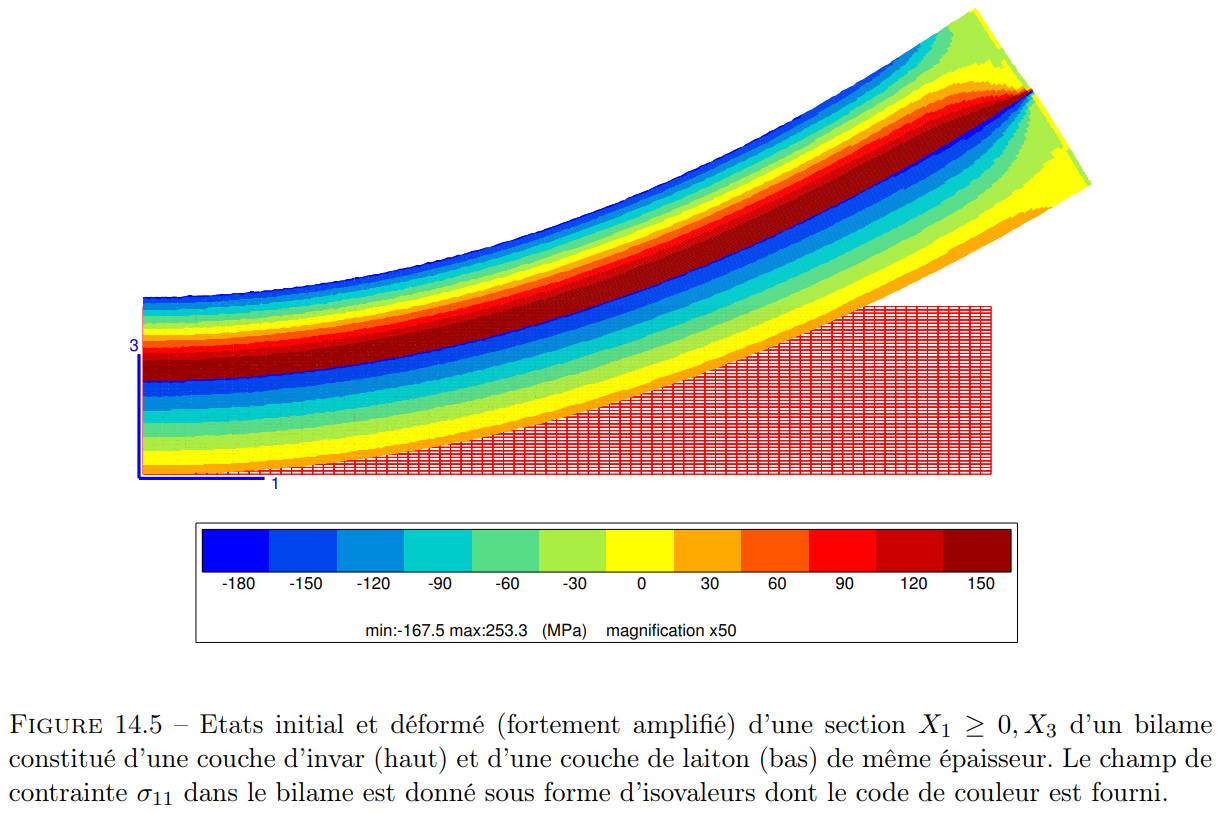
\includegraphics[scale=0.5]{imgs/simul_num.png}
    \end{figure}
\end{frame}

\subsection{Résolution du système}

\begin{frame}{Résolution du système}
    Le système précédent admet comme solution :
    $$A = 6\frac{M_fh_f}{M_sh_{s}^{2}}(\alpha_f-\alpha_s)(T-T_0)(1+\frac{h_f}{h_s})\Delta^{-1}$$
    $$\Delta = 1+4\frac{M_f}{M_s}\frac{h_f}{h_s}+6\frac{M_f}{M_s}\frac{h_f^2}{h_s^2}+4\frac{M_f}{M_s}\frac{h_f^3}{h_s^3}+\frac{M_f^2}{M_s^2}\frac{h_f^4}{h_s^4}$$
    $$C = (\alpha_s+4\alpha_f\frac{M_f}{M_s}\frac{h_f}{h_s}+3(\alpha_s+\alpha_f)\frac{M_f}{M_s}\frac{h_f^2}{h_s^2}+4\alpha_s\frac{M_f}{M_s}\frac{h_f^3}{h_s^3}+\alpha_f\frac{M_f^2}{M_s^2}\frac{h_f^4}{h_s^4})(T-T_0)\Delta^{-1}$$
\end{frame}

\subsection{Bilame de laiton et d'invar}

\begin{frame}{Application : bilame de laiton et d'invar}
    \textbf{\Large{Validité du contexte infinitésimal}}
    
    Pour ce bilame laiton/invar, $h_s = h_f = \frac{h}{2}$ et $\frac{M_f}{M_s} = 2$, d'où :
    $$\Delta = 1+4\cdot2\cdot1+6\cdot2\cdot1+4\cdot2\cdot1+2^{2}\cdot1 = 33$$
    $$A = \frac{8}{11}(\alpha_f-\alpha_s)\frac{T-T_0}{h_s}$$
    $$C = \frac{T-T_0}{11}(5\alpha_s+6\alpha_f)$$
    
    On doit avoir $||Grad(\underline{u})|| \ll 1$.
    $$\frac{\partial u_1}{\partial X_1} = A X_3+C,\; \frac{\partial u_1}{\partial X_3} = A X_1,\; \frac{\partial u_3}{\partial X_1} = -A X_1$$
    $$\frac{\partial u_3}{\partial X_3} = -\frac{2\nu}{1-\nu}(A X_3 + C) + \frac{1+\nu}{1-\nu}\alpha(T-T_0)$$
\end{frame}

\begin{frame}{Application : bilame de laiton et d'invar}
    \textbf{Conditions suffisantes :}
    \begin{itemize}
        \item $|\alpha_s(T-T_0)|\ll 1 \rightarrow$ contrôle de $|A X_3|$ et $|C|$
        \item $|\alpha_f(T-T_0)|\ll 1 \rightarrow$ contrôle de $|A X_3|$ et $|C|$
        \item $|(\alpha_s-\alpha_f)(T-T_0)|\frac{L}{h_s}\ll 1 \rightarrow$ contrôle de $|A X_1|$
    \end{itemize}
    Pour le laiton/invar :
    \begin{itemize}
        \item $|\alpha_s(T-T_0)|\approx19\cdot10^{-6}\cdot100\ll1$
        \item $|\alpha_f(T-T_0)|\approx1.2\cdot10^{-6}\cdot100\ll1$
        \item $\frac{L}{h_s}\ll \frac{1}{|(\alpha_s-\alpha_f)(T-T_0)|} \approx \frac{1}{17.8\cdot 10^{-4}}\approx 5\cdot 10^{-6}$
    \end{itemize}
\end{frame}

\begin{frame}{Application : bilame de laiton et d'invar}
    \textbf{\Large{Profils de déplacement}}
    
    \begin{itemize}
        \item A l'interface, en $X_3=0$:
    \end{itemize}
    \begin{figure}
        \centering
        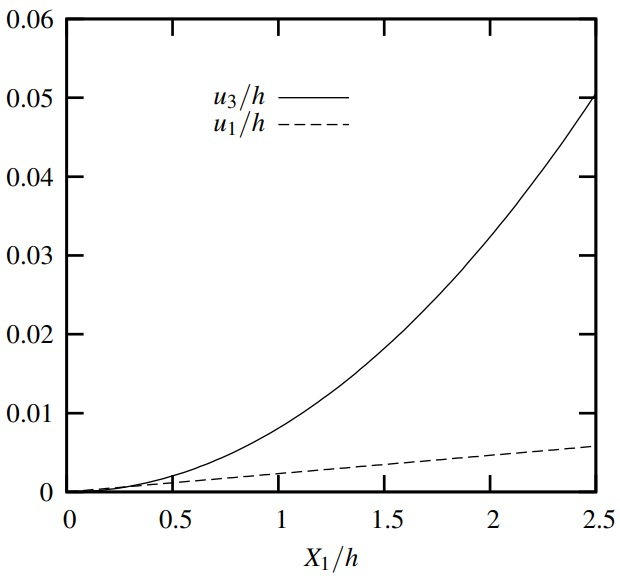
\includegraphics[scale=0.5]{imgs/graph1.jpg}
        \caption{Déplacements de l'interface du bicouche $X_3=0$}
    \end{figure}
\end{frame}

\begin{frame}{Application : bilame de laiton et d'invar}
    \textbf{\Large{Profils de déformation}}
    
    \begin{itemize}
        \item Sur l'axe $X_1=X_2=0$:
    \end{itemize}
    \begin{figure}
        \centering
        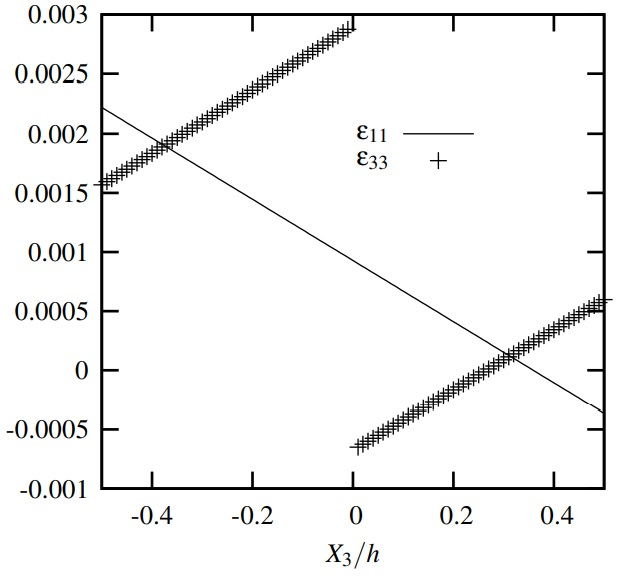
\includegraphics[scale=0.5]{imgs/graph2.jpg}
        \caption{Déformations le long de l'axe $X_1=X_2=0$}
    \end{figure}
\end{frame}

\begin{frame}{Application : bilame de laiton et d'invar}
    \textbf{\Large{Profils de contrainte}}
    
    \begin{itemize}
        \item Sur l'axe $X_1=X_2=0$:
    \end{itemize}
    \begin{figure}
        \centering
        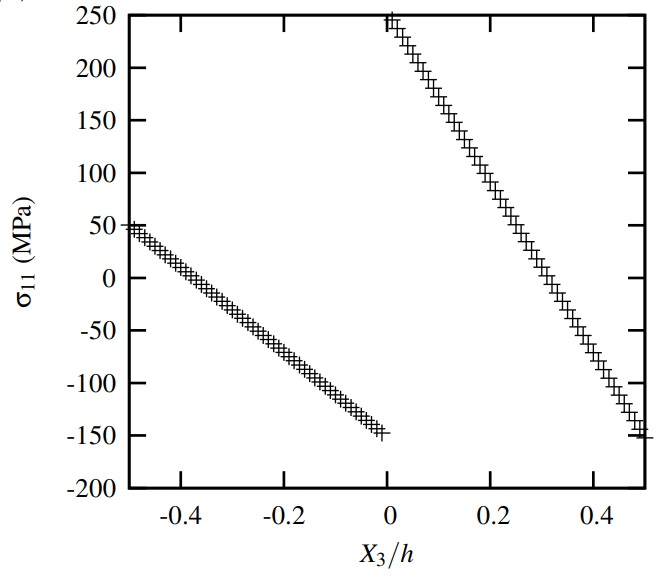
\includegraphics[scale=0.5]{imgs/graph3.jpg}
        \caption{Contraintes le long de l'axe $X_1=X_2=0$}
    \end{figure}
    Contrainte maximale atteinte pour $\frac{X_3}{h_s} = 0^+ : \sigma_{max} = 253 MPa$
\end{frame}

%------------------------------------------------
\section{Mécanique des microsystèmes} % Sections can be created in order to organize your presentation into discrete blocks, all sections and subsections are automatically printed in the table of contents as an overview of the talk
%------------------------------------------------

\subsection{La formule de Stoney} % A subsection can be created just before a set of slides with a common theme to further break down your presentation into chunks

\begin{frame}
    \frametitle{Contexte et rappels}
    \begin{itemize}
        \item Deux matériaux quelconques
        \item Petites déformations (HPP)
        \item $\bm{u} = (AX_1X_3 + CX_1)\bm{e_1} + (AX_2X_3 + CX_2)\bm{e_2} + (-\frac{A}{2}\left[X_1^2+X_2^2\right]-\frac{2\nu}{1-\nu}\left[\frac{A}{2}X_3^2+CX_3\right]+\frac{1+\nu}{1-\nu}\alpha\left[T-T_0\right]X_3)\bm{e_3}$
        \item $A = 6\frac{M_fh_f}{M_sh_s^2}(\alpha_f-\alpha_s)(T-T_0)(1+\frac{h_f}{h_s})\Delta^{-1}$
        \item $\Delta = 1+4\frac{M_fh_f}{M_sh_s}+6\frac{M_fh_f^2}{M_sh_s^2}+4\frac{M_fh_f^3}{M_sh_s^3}+\frac{M_f^2h_f^4}{M_s^2h_s^4}$
        \item $C = \Delta^{-1}(T-T_0)\left[\alpha_s + 4 \alpha_f \frac{M_fh_f}{M_sh_s} + 3 (\alpha_s + \alpha_f)\frac{M_fh_f^2}{M_sh_s^2} + 4\alpha_s \frac{M_fh_f^3}{M_sh_s^3} + \alpha_f \frac{M_f^2h_f^4}{M_s^2h_s^4}  \right]$
    \end{itemize}
\end{frame}

% 30s
    
\begin{frame}
    \frametitle{La formule de Stoney (1909)}
    
    \begin{figure}
        \centering
        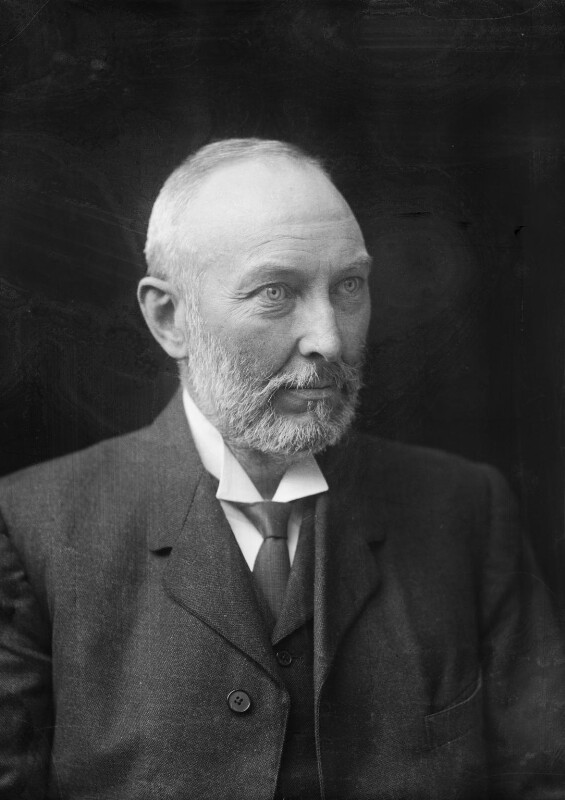
\includegraphics[scale=0.07]{imgs/stoney.jpg}
        \caption{George Gerald Stoney (1863-1942)}
    \end{figure}

    \begin{itemize}
        \item Supposons que $\frac{h_s}{h_f} << 1$
        \item Quelle est la courbure $c$ prise par l'ensemble ?
    \end{itemize}
    
    \begin{figure}
        \centering
        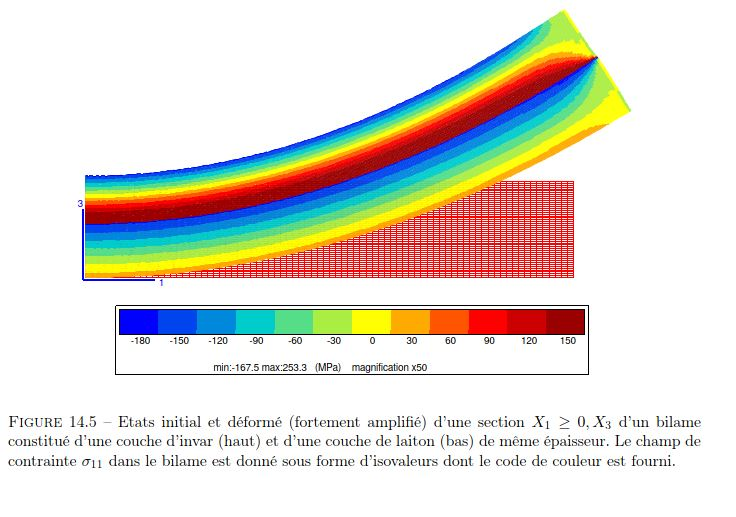
\includegraphics[scale=0.2]{imgs/deformation.JPG}
        \caption{Résultat de simulation}
    \end{figure}
    
\end{frame}


% 1m

\begin{frame}
    \frametitle{La formule de Stoney (1909)}

    \begin{itemize}
        \item $c = 6\frac{M_fh_f}{M_sh_s^2}(\alpha_s-\alpha_f)(T-T_0)$ si $M_fh_f << M_sh_s$ 
        \item Dans les autres directions ? Courbure nulle ou parabolique
        \item Permet de prévoir la déformation de l'ensemble, en combinant ls caractéristiques géométriques et les propriétés mécaniques des couches
    \end{itemize}
    
    \begin{figure}
        \centering
        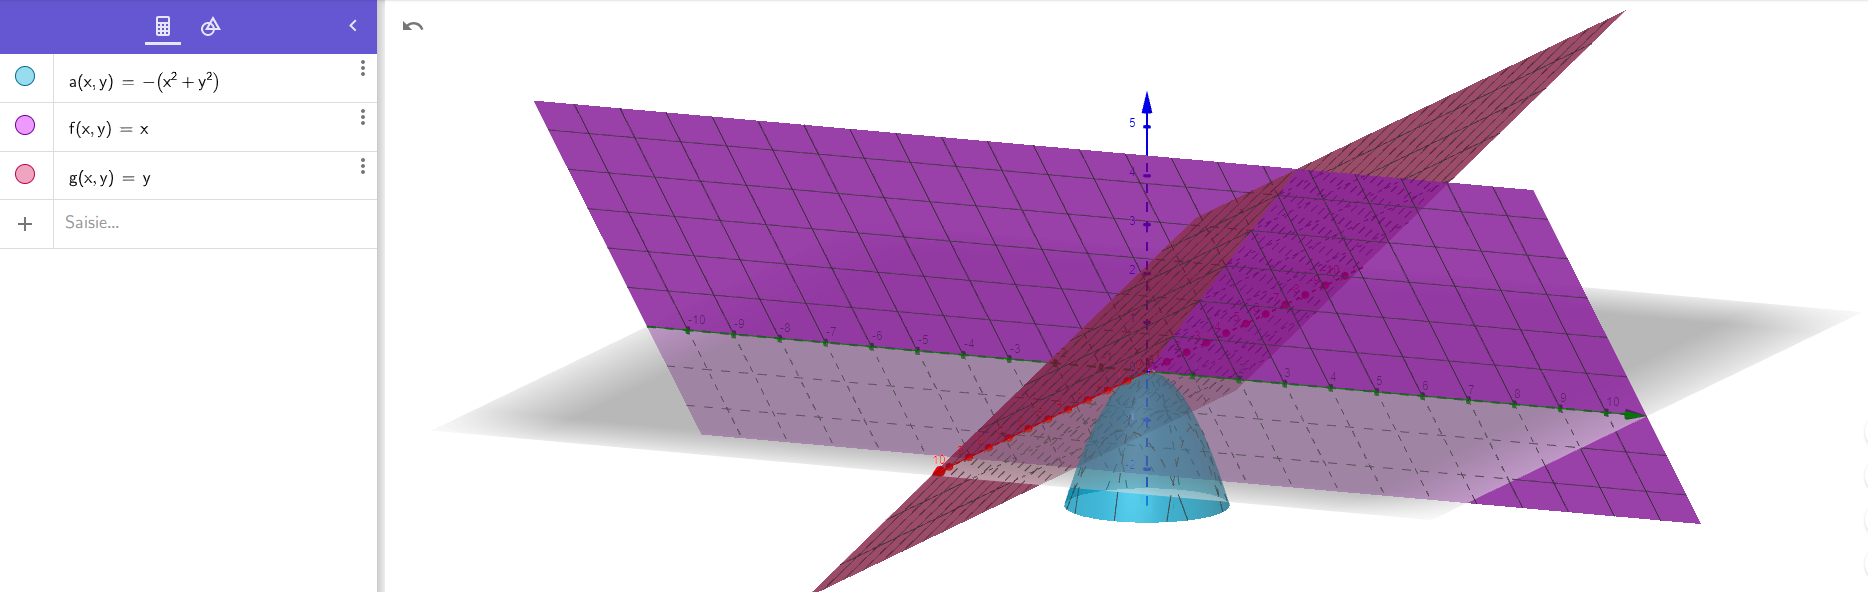
\includegraphics[scale=0.25]{imgs/courbes.png}
        \caption{Paraboloïde de révolution et hyperplans}
    \end{figure}
    
\end{frame}

% 4m15

\begin{frame}
    \frametitle{La formule de Stoney (1909)}

    \begin{itemize}
        \item Qu'évoquait l'article de Stoney ?
        \item Une formule estimant sous certaines conditions (précédemment évoquées) pour déterminer en mesurant la tension et la courbure la couche de nickel déposée sur une électrode 
        \item Reliait la valeur des contraintes à la courbure de l'électrode avec son dépôt
        \item Formule 2D améliorée par Berry en 1988
    \end{itemize}
    
\end{frame}

% 4m45

\begin{frame}
\frametitle{Expérience sommaire : présentation}
\begin{itemize}
    \item Découper des bandes (8 cm par 1 cm environ)
    \item Feuille d'aluminium : $\alpha_f = 23 \times 10^{-6} K^{-1}$, $h_f = 0.02 mm$, $E_f = 62 GPa$, $\nu_f = 0.35$
    \item Papier bristol : $\alpha_s = 3 \times 10^{-6} K^{-1}$, $h_s = 0.3 mm$, $E_s = 3 GPa$, $\nu_s = 0.2$
    \item Colle pour fixer les deux morceaux
    \item Bougie : $T = 200$ °C (juste en-dessous de la température d'auto-inflammation du papier) et $T_0 = 25$ °C
    \item C'est parti !
\end{itemize}
\end{frame}

% 6m

\begin{frame}
\frametitle{Expérience sommaire : résultats}
    \begin{itemize}
        \item Une des deux faces se dilate sous l'effet de la chaleur
        \item On remarque que c'est l'aluminium qui est sur la face interne de la courbure. 
        \item On peut chercher à vérifier le signe de la courbure dans la formule de Stoney, même si la deuxième hypothèse $M_f h_f << M_s h_s$ n'est pas vraiment vérifiée :
        \begin{itemize}    
            \item $T-T_0 > 0$
            \item $\alpha_s - \alpha_f < 0$
            \item Donc $c < 0$ (la courbure est vers le bas)
        \end{itemize}
        \item Diversité des applications de cet effet (ici, Stoney, électronique)
    \end{itemize}
\end{frame}

%6m30


\subsection{Contraintes dans un film mince sur un substrat} % A subsection can be created just before a set of slides with a common theme to further break down your presentation into chunks

\begin{frame}
\frametitle{Forme simplifiée des contraintes sous les hypothèses de Stoney}
\begin{itemize}
    \item Contrainte moyenne : $\bar{\sigma}_{11}=\frac{1}{h}\int\sigma_{11}\rm{d}X_3$
    \item Développons au premier ordre $\Delta$, $C$ et $A$
    \item $\sigma_{11}^f=M_f(AX_3+C-\alpha_f(T-T_0))$
    \item $\sigma_{11}^s=M_s(AX_3+C-\alpha_s(T-T_0))$
\end{itemize}
\end{frame}

% 8m

\begin{frame}
    \frametitle{Forme simplifiée des contraintes sous les hypothèses de Stoney}
    \begin{itemize}
        \item Par équi-biaxialité, $\bar{\sigma}_{11}^f=\bar{\sigma}_{22}^f=M_f(\alpha_s-\alpha_f)(T-T_0)$, ce qui est un résultat remarquable (ne dépend pas de la géométrie ni des propriétés élastiques du substrat, que de propriétés thermoélastiques du film et du désaccord de dilatation)
        \item De même, $\bar{\sigma}_{11}^s=\bar{\sigma}_{22}^s=M_f\frac{h_f}{h_s}(\alpha_f-\alpha_s)(T-T_0)$
        \item La contrainte moyenne est donc nulle (cohérent car il n'y a pas de chargement extérieur et l'on est en statique, que des contraintes locales à l'intérieur)
        \item Quelle est la fibre neutre ?
    \end{itemize}
\end{frame}

% 9m15

\begin{frame}
    \frametitle{Fibre neutre}
    \begin{itemize}
        \item $\sigma_{11}^s=0 \implies X_3 \simeq \frac{-2h_s}{3}$ (cohérent, bien dans le substrat, car contrainte constante dans le film)
        \item Confirmation par représentation graphique et l'article de Stoney
    \end{itemize}
\end{frame}

% 10m



\subsection{Contraintes résiduelles dans un dépôt d'aluminium sur un substrat de silicium} 
\subsection{Contraintes d'épitaxie} 


\begin{frame}
    \Huge{\centerline{Merci ! Des questions ?}}
\end{frame}
    

%------------------------------------------------
%------------------------------------------------

% \begin{frame}
% \frametitle{Blocks of Highlighted Text}
% \begin{block}{Block 1}
% Lorem ipsum dolor sit amet, consectetur adipiscing elit. Integer lectus nisl, ultricies in feugiat rutrum, porttitor sit amet augue. Aliquam ut tortor mauris. Sed volutpat ante purus, quis accumsan dolor.
% \end{block}

% \begin{block}{Block 2}
% Pellentesque sed tellus purus. Class aptent taciti sociosqu ad litora torquent per conubia nostra, per inceptos himenaeos. Vestibulum quis magna at risus dictum tempor eu vitae velit.
% \end{block}

% \begin{block}{Block 3}
% Suspendisse tincidunt sagittis gravida. Curabitur condimentum, enim sed venenatis rutrum, ipsum neque consectetur orci, sed blandit justo nisi ac lacus.
% \end{block}
% \end{frame}

%------------------------------------------------

% \begin{frame}
% \frametitle{Multiple Columns}
% \begin{columns}[c] % The "c" option specifies centered vertical alignment while the "t" option is used for top vertical alignment

% \column{.45\textwidth} % Left column and width
% \textbf{Heading}
% \begin{enumerate}
% \item Statement
% \item Explanation
% \item Example
% \end{enumerate}

% \column{.5\textwidth} % Right column and width
% Lorem ipsum dolor sit amet, consectetur adipiscing elit. Integer lectus nisl, ultricies in feugiat rutrum, porttitor sit amet augue. Aliquam ut tortor mauris. Sed volutpat ante purus, quis accumsan dolor.

% \end{columns}
% \end{frame}

%------------------------------------------------
% \section{Second Section}
%------------------------------------------------

% \begin{frame}
% \frametitle{Table}
% \begin{table}
% \begin{tabular}{l l l}
% \toprule
% \textbf{Treatments} & \textbf{Response 1} & \textbf{Response 2}\\
% \midrule
% Treatment 1 & 0.0003262 & 0.562 \\
% Treatment 2 & 0.0015681 & 0.910 \\
% Treatment 3 & 0.0009271 & 0.296 \\
% \bottomrule
% \end{tabular}
% \caption{Table caption}
% \end{table}
% \end{frame}

%------------------------------------------------

% \begin{frame}
% \frametitle{Theorem}
% \begin{theorem}[Mass--energy equivalence]
% $E = mc^2$
% \end{theorem}
% \end{frame}

%------------------------------------------------

% \begin{frame}[fragile] % Need to use the fragile option when verbatim is used in the slide
% \frametitle{Verbatim}
% \begin{example}[Theorem Slide Code]
% \begin{verbatim}
% \begin{frame}
% \frametitle{Theorem}
% \begin{theorem}[Mass--energy equivalence]
% $E = mc^2$
% \end{theorem}
% \end{frame}\end{verbatim}
% \end{example}
% \end{frame}

%------------------------------------------------

% \begin{frame}
% \frametitle{Figure}
% Uncomment the code on this slide to include your own image from the same directory as the template .TeX file.
% %\begin{figure}
% %\includegraphics[width=0.8\linewidth]{test}
% %\end{figure}
% \end{frame}

%------------------------------------------------

% \begin{frame}[fragile] % Need to use the fragile option when verbatim is used in the slide
% \frametitle{Citation}
% An example of the \verb|\cite| command to cite within the presentation:\\~

% This statement requires citation \cite{p1}.
% \end{frame}

%------------------------------------------------

% \begin{frame}
% \frametitle{References}
% \footnotesize{
% \begin{thebibliography}{99} % Beamer does not support BibTeX so references must be inserted manually as below
% \bibitem[Smith, 2012]{p1} John Smith (2012)
% \newblock Title of the publication
% \newblock \emph{Journal Name} 12(3), 45 -- 678.
% \end{thebibliography}
% }
% \end{frame}

%------------------------------------------------

%----------------------------------------------------------------------------------------

\end{document} 